\documentclass[11pt]{article}
\usepackage{amsmath,textcomp,amssymb,graphicx,cancel}
\usepackage{gensymb}
\usepackage[margin=1in]{geometry}
\usepackage{pgfplots}
\pgfplotsset{width=7cm,compat=1.8}
\usepackage[colorlinks, urlcolor=blue]{hyperref}
\usepackage{tikz}
\usepackage{epigraph}

%\setlength\parindent{24pt}

\def\Name{Zackery Field}  % Your name
\def\Session{Fall 2013} %Semester

\title{BIOE147 -- Fall 2013 -- PS2}
\author{\Name}
\markboth{BIOE147 \Session \Name}{\Name -- PS2}
\pagestyle{myheadings}

\renewcommand\epigraphflush{flushright}
\renewcommand\epigraphsize{\normalsize}
\setlength\epigraphwidth{0.7\textwidth}

\definecolor{titlepagecolor}{cmyk}{1,.60,0,.40}

\begin{document}
% \sffamily
% \fontspec
%   []
%   {SourceCodePro-Regular.otf}
\maketitle
\section*{1. Logic Gates and Biology}

The NAND gate is often the only one used in electronic circuits. One of the main reasons for this is that the NAND gate is functionally complete, which means that all other logic gates can be represented by only NAND gates.

\begin{itemize}

 \item[{\bf (a.)}]Write a truth table for the following NAND gate circuits and show what gate they represent:

{\centering
  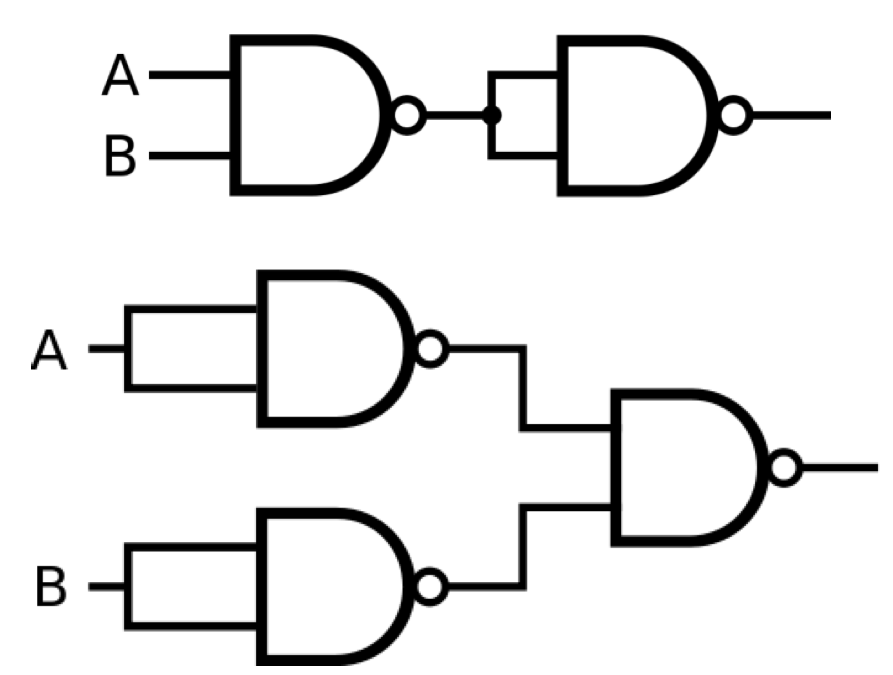
\includegraphics[scale=0.3, trim = 0mm 0mm 7mm 0mm, clip]{ps2_logic.png}\par
 }
{
  \centering
  \begin{tabular}{ c | c | c | c | c }
    A & B & $\sim(A\wedge B)$ & G1($A\wedge B$) & G2($A\vee B$) \\
  \hline
  1 & 1 & 0 & 1 & 1 \\
  1 & 0 & 1 & 0 & 1 \\
  0 & 1 & 1 & 0 & 1 \\
  0 & 0 & 1 & 0 & 0 \\
  \end{tabular}
  \par
}

\item[{\bf (b.)}] Design a biological system that performs the function of a NAND gate and the two gates above. Use only transcriptional regulation and use only the specific biological parts covered in the course.

  \begin{itemize}
\item {\bf AND:}
In order to implement the AND architecture we can using a two repressors. Let $p_1, p_2$ be two constitutive promoters and $p_3,p_4$ be two repressible promoters, $r_3,r_4$ be the repressor protein of $p_3,p_4$, and $s_3,s_4$ be the two small molecule repression inhibitors. 

$p_1$ promotes the transcription of $r_3$, and $p_2$ promotes the transcription of $r_4$. 
The reporter $R$ is being repressed by both $p_3$ and $p_4$. 
It is assumed that the repression of either $p_3$ or $p_4$ is enough to repress the transcription of $R$. 
So, only the presence of both $s_3$ {\bf and} $s_4$ will activate transcription of the reporter. Options for repressible systems are LacO/LacI and cl-ts. 
The first gate in the figure is the equivalent of an AND gate.

\item {\bf NAND:}  The NAND gate can be created by implementing an AND gate and then simply flipping the output using a repressor.
Starting with the AND gate above, make the output be another repressor protein $r_5$ (instead of the reporter $R$). 
This repressor protein will act on on $p_5$ and then repress the transcription of $R$. This will ensure that $R$ is only repressed when both $s_3$ {\bf and} $s_4$ are present.
Since LacI/LacO and cl-ts were recommended for the AND gate, tetR can be used as the $p_5/r_5$ system.

\item {\bf OR:} The second gate in the figure is an OR gate. To construct this gate you can make two orthogonal circuits that both regulate the production of the same reporter $R$ (GFP). Each of these circuits will act in the same way. 
Let $p$ be the repressor, $r$ be the repressor protein that modulates $p$, and $s$ be the small molecule inhibitor that inactives $r$. The repressor proteins for each of the circuits will be transcribed constitutively.
 Therefore, the presence of either the $s$ for one circuit {\bf or} the other (or {\bf both}) will activate the transcription of the reporter $R$.
  \end{itemize}

\item[{\bf (c.)}] Could we construct the two gates above using only the NAND gate in biological systems? Is it feasible to utilize the NAND only architecture in biological systems?

With the materials that we have been restricted to thusfar, no. 
If all parts known were available it may be feasible to construct the two example circuits, but beyond that it would not be feasible to construct larger systems with NAND only architecture.
 A key reason that NAND only architecture works in EE applications is that you can construct a many orthogonal NAND gates with ease, while in biology you do not have that luxury.

\end{itemize}

\section*{2. Time Delays in Circuits}

\begin{itemize}

\item[{\bf (a.)}] Fill out the truth table and timing diagram. Assume all gates have a delay of one time unit. 

{\centering
  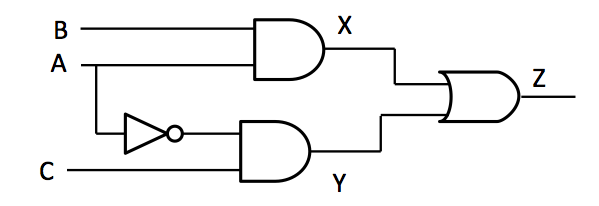
\includegraphics[scale=0.5, trim = 0mm 0mm 7mm 0mm, clip]{ps_2_timing.png}\par
 }
{
  \centering
  \begin{tabular}{ c | c | c | c | c | c }
    A & B & C & X & Y & Z\\
  \hline
  0 & 0 & 0 & 0 & 0 & 0\\  
  0 & 0 & 1 & 0 & 1 & 1\\
  0 & 1 & 0 & 0 & 0 & 0\\
  0 & 1 & 1 & 0 & 1 & 1\\
  1 & 0 & 0 & 0 & 0 & 0\\
  1 & 0 & 1 & 0 & 0 & 0\\
  1 & 1 & 0 & 1 & 0 & 1\\
  1 & 1 & 1 & 1 & 0 & 1\\
  \end{tabular}
  \par
}

{ 
  \centering
  \begin{tikzpicture}
    # Grid
    \draw[step = 0.5, color=gray, line width=0.5pt] (-0.5,-0.5) grid (12,5);
    \node at (-0.25,4.75) {A};
    \node at (-0.25,3.75) {B};
    \node at (-0.25,2.75) {C};
    \node at (-0.25,1.75) {X};
    \node at (-0.25,0.75) {Y};
    \node at (-0.25,-0.25) {Z};
    \draw (0,-0.5) -- (0,5);
    # Initial Phase
    \draw[line width=2pt] (0,5) -- (3,5);#A
    \draw[line width=2pt] (0,4) -- (12,4);#B
    \draw[line width=2pt] (0,3) -- (12,3);#C
    \draw[line width=2pt] (0,2) -- (3,2);#X
    \draw[line width=2pt] (0,0.5) -- (3,0.5);#Y
    \draw[line width=2pt] (0,0) -- (3,0);#Z
    # Change happens in A
    \draw[line width=2pt] (3,5) -- (3,4.5);#A
    \draw[line width=2pt] (3,4.5) -- (12,4.5);#A
    # No chage recognition till 4
    \draw[line width=2pt] (3,2) -- (4,2);#X
    \draw[line width=2pt] (3,0.5) -- (5,0.5);#Y
    \draw[line width=2pt] (3,0) -- (5,0);#Z
    # X shuts down
    \draw[line width=2pt] (4,2) -- (4,1.5);#X
    \draw[line width=2pt] (4,1.5) -- (12,1.5);#X
    # Y takes an extra step to react
    \draw[line width=2pt] (5,0.5) -- (5,1);#Y
    \draw[line width=2pt] (5,1) -- (12,1);#Y
    # Z fails
    \draw[line width=2pt] (5,0) -- (5,-0.5);#Z
    \draw[line width=2pt] (5,-0.5) -- (6,-0.5);#Z
    \draw[line width=2pt] (6,-0.5) -- (6,0);#Z
    \draw[line width=2pt] (6,0) -- (12,0);#Z
 \end{tikzpicture}
}



\item[{\bf (b.)}] What happened to output Z when A switched signals?

There was a time delay of one time step when X turned to the 0-state, and a time step of two when Y turned to the  1-state. This meant that there was one time unit where both X and Y were in the 0-state, and therefore for the time step following, Z was also in the 0-state. 
If the system is designed for X and Y to fluctuate while Z maintains the 1-state invariant then the time delay observed that puts Z in the 0-state would cause issue with whatever behaved with the expectation that Z would alwasys be in the 1-state.
\item[{\bf (c.)}] Redesign the circuit above to eliminate the problem caused by the delay. 

An addition of a buffer gate between A and the X gate would stall the A signal for another time step as Y switched from the 0-state to the 1-state. This would eliminate the one time step gap where Z is in the 0-state.

\item[{\bf (d.)}] If there is no A in the system at time 0 and its expression is turned on, find how much time it would take for the cell to begin expressing GFP.


{
  \centering
  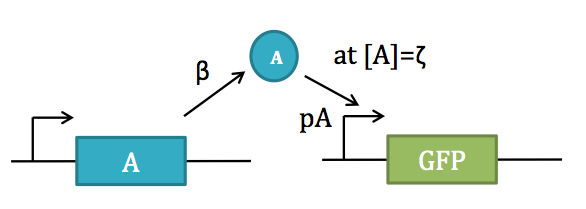
\includegraphics[scale=0.5, trim = 0mm 0mm 7mm 0mm, clip]{ps_2_timebio.png}\par
 }
 
\begin{equation*}
  \begin{align}
  \frac{d[A]}{dt}&=\beta - \alpha\\
  [A] &= \exp^{(\beta-\alpha)t}\\
  t &= \frac{\ln{\zeta}}{\beta-\alpha}
  \end{align}
\end{equation*}

\end{itemize}

\newpage

\section*{3. Cooperative binding and part definitions}

{
  \centering
  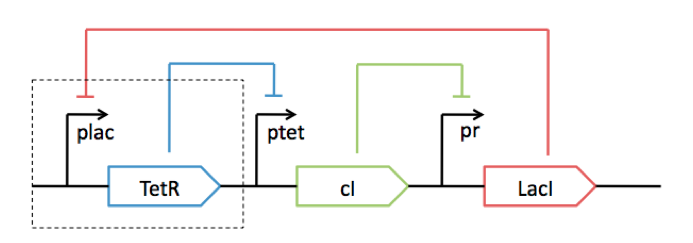
\includegraphics[scale=0.5, trim = 0mm 0mm 7mm 0mm, clip]{ps_2_repress.png}\par
 }
\begin{itemize}
\item[{\bf (a.)}]
\end{itemize}

\section*{4. Heat Dissipation in Bacteria}

\begin{itemize}
\item[(a.)]
\end{itemize}
\end{document}
